\documentclass[a4paper]{article}
\setlength{\headheight}{1.1\baselineskip}
%\usepackage[margin=1.0 in]{geometry}
%\renewcommand{\baselinestretch}{1.5}

\usepackage[english]{babel}
\usepackage[utf8]{inputenc}
% package for including graphics with figure-environment
\usepackage{graphicx}
\usepackage{hyperref}
% colors for hyperlinks
% colored borders (false) colored text (true)
\hypersetup{colorlinks=true,citecolor=black,filecolor=black,linkcolor=black,urlcolor=black}

% package for bibliography
%\usepackage[authoryear,round]{natbib}
% package for expectation signs
\usepackage{amsmath,amssymb,mathtools,bm,etoolbox}
%\documentclass[a4paper,11pt]{report} 
\usepackage{breqn}
\usepackage{amsmath}
\usepackage{enumitem} 
\usepackage{amsmath, amsthm, amssymb}
\usepackage{amsmath}
\newcommand{\abs}[1]{ \left\lvert#1\right\rvert} 
\newcommand{\norm}[1]{\left\lVert#1\right\rVert}
% package for header
\usepackage[automark]{scrpage2}
\pagestyle{scrheadings}
\ihead[]{Isa Marques, Xi Sun, Xueying Liu}
\ohead[]{\today}
\cfoot[]{\pagemark} 
\setheadsepline[122mm]{0.3mm}
\usepackage{csquotes}



% some more packages enabling table and figure production
\usepackage{float, afterpage, rotating, graphicx}
\usepackage{epstopdf}
\usepackage{longtable, booktabs, tabularx}
\usepackage{fancyvrb, moreverb, relsize}
\usepackage{eurosym, calc, chngcntr}
\usepackage{caption}
\usepackage{mdwlist}
\usepackage{xfrac}
\usepackage{setspace}
\usepackage{xcolor}
\usepackage{multirow}
%\usepackage{booktabs}


% packages for bibliography
\usepackage[backend=biber, natbib=true,style=numeric]{biblatex}
\AtBeginDocument{\toggletrue{blx@useprefix}}
\AtBeginBibliography{\togglefalse{blx@useprefix}}
\setlength{\bibitemsep}{1.5ex}
\addbibresource{refs.bib}




\begin{document}
	\title{
	%\begin{figure}[!ht]
	%	\flushleft
	%		\includegraphics[width=0.7\textwidth]{logo.eps}
	%\end{figure}
	\vspace{1cm}
	\Huge \textbf{ Semiparametric Single Index Models }\\ \Large Ichimura's and Klein and Spady's methods \\
	}
	
	\vspace{1cm}
	
	% if you are the only author, you might use the following
	% \author{Name of student}	
	
	% Insert here your name and correct mail address
	\author{\Large \href{mailto:first.student@smail.fh-koeln.de}{Isa Marques}\and \Large \href{mailto:second.student@smail.fh-koeln.de}{Xi Sun} \and \Large \href{mailto:second.student@smail.fh-koeln.de}{Xueying Liu}
	\vspace{1cm}}
	
	% name of the course and module
	\date{
	\large University of Bonn \\ Project Module in Econometrics and Statistics\\ 
	\vspace{0.8cm}
	\large Prof. Dr. Kneip \\
	\large Prof. Dr. Liebl \\
	\vspace{1cm}
	\today
	}

	\maketitle
	\setlength{\parindent}{0pt}

\vspace{2cm}
\begin{abstract}


\end{abstract}
%	\newpage
%	\tableofcontents
	\newpage
	
\section{Introduction} % (fold)
\label{sec:introduction}
THIS SECTION WILL WRITTEN WHEN THE APPLIED PART IS DONE.
%Say who did what.



%Semiparametric single index models are widely applied in economic research. Applications range from finance to labor economics.

% section introduction (end)
%The main focus of this paper is Ichimura's semiparametric model. In section 4 the identification conditions necessary for uniquely determining $\beta_0$ and $g(\cdot)$ in semiparametric models are presented.  Furthermore, Ichimura's solution will be analyzed in detail in section 5. The latter section briefly explains the weight function and bandwidth selection. As a comparison to Ichimura's method, Klein and Spady's (1993) semiparametric binary choice model will be explained concisely in section 6. Finally, in section 6 the two models are compared in both a theoretical and applied perspective.



\section{Empirical Application} % (fold)
\label{sec:Empirical Application}

This section presents an empirical application on gender recognition by voice using the aforementioned statistical methods. A comparison with simple logistic regression is also made. 

The dataset we used is the pre-processed Gender Recognition by Voice and Speech Analysis dataset, a publicly available dataset from online resources containing 3,168 recorded voice samples by 1584 male and 1584 female speakers. 21 independent variables of acoustic properties of voice and 1 binary dependent indicator variable for gender are included in the dataset. More information regarding the dataset can be found in the appendix.  

As a first step, we removed three variables that have shown to cause multicollinearity problem,  namely; IQR, centroid, and dfrange. Next, the dataset is split into training sample for estimation of parameters, and test sample for prediction using estimated parameters. 70\% of the data are randomly selected into the training sample, with the remaining 30\% left for the test sample. 

For estimation, we use the pre-implemented np-package in R (Racine and Hayfield, 2008) \cite{[28]} for computational simplicity. In our self-implemented Ichimura method and Klein and Spady method, we employed grid-search in the minimization process for equation (9) and (14), which is also the method proposed by Ichimura (1993) \cite{[6]}. The minimization results are highly dependent on the specification of the grid for each independent variables and an appropriate resolution of the grid is necessary for precise results. As such, grid-search method suffers from the curse of dimensionality. Numerical approximation becomes infeasible in our case as the data contains 18 independent variables. We therefore decided to use the np-package which employs the $npksum()$ and $nlm()$ minimization procedures in R with multiple starting values to best avoid local minima. A comparison with logistic regression is also done using the logistic regression routine pre-implemented in R. 

The prediction results and the true values are plotted in figure 2. A comparison of in-sample and prediction accuracy rate and approximate calculation time are also presented in table 2. The accuracy rate is defined as ratio of correct gender prediction to the total number of data points.

\begin{table}
    \centering
	\begin{center}
	\begin{tabular}{  m{2cm} | m{3cm} & m{3cm} & m{3cm} |}
	  & Logistic Regression & Ichimura Method & Klein-Spady Method

	\tabularnewline
	\midrule

	Approximate calculation time & $<$ 1 second & $>$ 3 hours & $>$ 3 hours
	\tabularnewline
	\midrule

	In-sample Accuracy Rate (training sample) & 0.971145 & 0.974752 & 0.976104
	\tabularnewline
	\midrule

	Prediction Accuracy Rate (test sample) & 0.978947 &  0.977894 & 0.981052 
	\tabularnewline
	\bottomrule
	\end{tabular}
	\end{center}
	\caption {Estimation time and accuracy rate}
\end{table}

\bigskip
\bigbreak

\begin{figure}[H]

  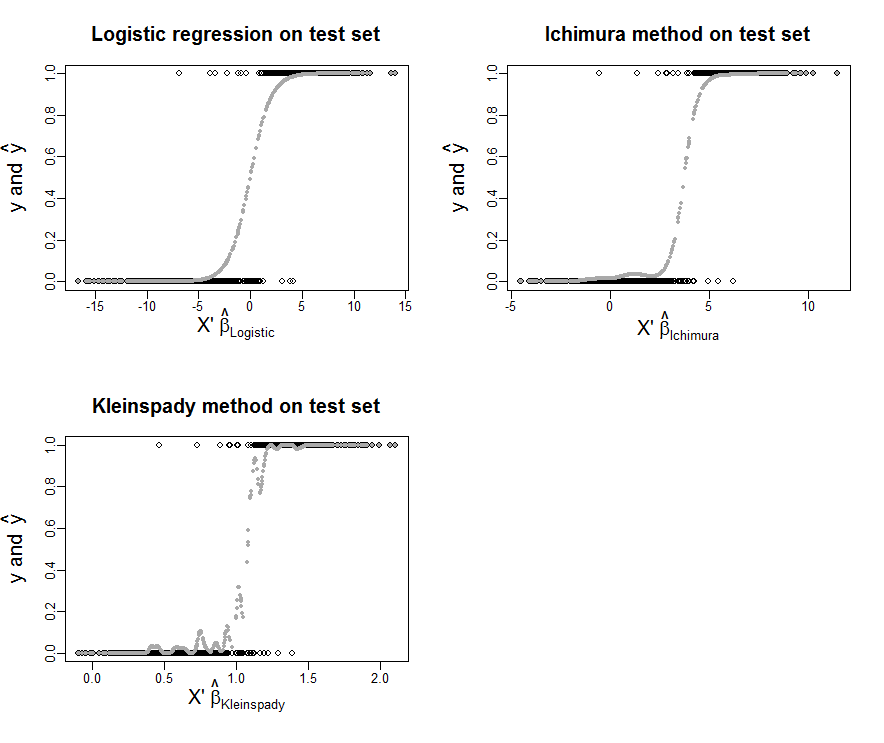
\includegraphics[width=\linewidth]{figure2.png}
 
  \label{fig: Plot of estimates on test sample}
  \caption{Plot of Estimates on Test Sample}
\end{figure}

From Table 2 and Figure 2, we could conclude that the logistic regression would be the preferred method in this case since the improvement in accuracy rate by using semi-parametric methods are minimum while the calculation time increases significantly. However, this could be due to the fact that the underlying data fit the logistic distribution better, and thus this comparison should not be generalized to other datasets. 

We also take note of the two peculiar features of the results. First, the accuracy rate is higher for test sample than in-sample accuracy rate. As the difference is relatively small, we postulate that this could be random and of no particular significance. Moreover, the fact that the training sample contains 3.5 times more data points than the test sample could exacerbate the random effect. The second feature is that the result graph from Klein and Spady method is not very smooth. This could be due to a problem with band-width selection included in the np-package (Racine and Hayfield, 2008) \cite{[28]} or the minimization process. However, as the result is not significantly worse than the other estimators, actually slightly better, we do not think that this should be of great concern.


\newpage 

\section{Appendix} % (fold)
\label{sec:appendix}

\subsection{List of Variables}
The following list shows the 21 independent variables and 1 binary gender indicator contained in the dataset.

\begin{center}
\begin{tabular}{ m{5em} | m{10cm}}
\toprule
Variable Name & Description
\tabularnewline
\midrule
meanfreq & mean frequency (in kHz)
\tabularnewline
sd & standard deviation of frequency
\tabularnewline
median & median frequency (in kHz)
\tabularnewline
Q25 & first quantile (in kHz)
\tabularnewline
Q75 & third quantile (in kHz)
\tabularnewline
IQR & interquartile range (in kHz)
\tabularnewline
skew & skewness
\tabularnewline
kurt & kurtosis
\tabularnewline
sp.ent & spectral antropy
\tabularnewline
sfm & spectral flatness
\tabularnewline
mode & mode frequency
\tabularnewline
centroid & frequency centroid
\tabularnewline
peakf & peak frequency (frequency with highest energy)
\tabularnewline
meanfun & average of fundamental frequency measured across acoustic signal
\tabularnewline
minfun & minimum fundamental frequency measured across acoustic signal
\tabularnewline
maxfun & maximum fundamental frequency measured across acoustic signal 
\tabularnewline
meandom & average of dominant frequency measured across acoustic signal 
\tabularnewline
mindom & minimum of dominant frequency measured across acoustic signal 
\tabularnewline
maxdom & maximum of dominant frequency measured across acoustic signal 
\tabularnewline
dfrange & range of dominant frequency measured across acoustic signal 
\tabularnewline
modindx & modulation index. Calculated as the accumulated absolute difference between adjacent measurements of fundamental frequencies divided by the frequency range 
\tabularnewline
label & male or female
\tabularnewline

\bottomrule
\end{tabular}
\end{center}


\section{Bibliography} % (fold)
\label{sec:Bibliography}


\nocite{*}
\printbibliography[heading=none]

\end{document}